\documentclass[ignorenonframetext]{beamer} 

\usepackage[utf8]{inputenc} 
\usepackage{amsmath} 
\usepackage{amsfonts} 
\usepackage{amssymb} 
\usepackage[font=small]{caption} 



\mode<presentation> 
{ 
  \usetheme{Singapore} 
  \usecolortheme[named=darkgray]{structure} 

} 


\usepackage[]{algorithm2e}
\renewcommand{\figurename}{Figure}
%Standard Angaben
\author{Andrej}
\title{Foobar}
\date{\today}
\begin{document}
%---------------------------------------------1 FOLIE ---------------------------------------------
\section{}
\begin{frame}
\frametitle{

\begin{huge}
Desert Ant Adaptive Navigation
\end{huge}

}
\ \\
\ \\
\ \\

\begin{center}

Presentation 15th of December 2015\\
\ \\
\ \\
\ \\
\begin{LARGE}
Ants in the Pants\\
\end{LARGE}
Florian Hasler, Matthias Heinzmann, Andreas Urech, Dominik Werner

\end{center}

\end{frame}












\section{Introduction}
\subsection{What is it all about?}
%---------------------------------------------2 FOLIE ---------------------------------------------














\begin{frame} 
\frametitle{What is it all about?}



\only<1>{
 \begin{figure}[H]
 \centering
 \includegraphics[scale=0.7]{./Pics/meisi.png} 
 \caption{Cataglyphis fortis \footnote{http://www.lambrinos.ch December 5th 2015} \label{fig:Variance} }
 \end{figure}  
\begin{center} 
\end{center} 
}












\only<2>{
 \begin{figure}[H]
 \centering
 \includegraphics[scale=0.6]{./Pics/WhatAbout.png} 
 \caption{Foraging walks Wehner2003 \label{fig:Variancea} }
 \end{figure} 
\begin{center} 
\end{center} 
}







\only<3>{\begin{itemize}
\item one ant,  one prey $\rightarrow$ no further communication needed

\end{itemize}
 \begin{figure}[H]
 \centering
 \includegraphics[scale=0.6]{./Pics/WhatAbout.png} 
 \caption{Foraging walks Wehner2003 \label{fig:Variancea} }
 \end{figure} 
\begin{center} 
\end{center} 
}

\only<4>{\begin{itemize}
\item one ant,  one prey $\rightarrow$ no further communication needed
\item Why is time, hence the shortest way back so crucial?

\end{itemize}
 \begin{figure}[H]
 \centering
 \includegraphics[scale=0.6]{./Pics/WhatAbout.png} 
 \caption{Foraging walks Wehner2003} \label{fig:Variancea}
 \end{figure} 
\begin{center} 
\end{center} 
}








\only<5>{\begin{itemize}
\item one ant,  one prey $\rightarrow$ no further communication needed
\item Why is time, hence the shortest way back so crucial?
\item Distances in relation to ant's size.\\
Speed of cataglyphis fortis $\approx 1 \frac{m}{s}$
\end{itemize}
 \begin{figure}[H]
 \centering
 \includegraphics[scale=0.6]{./Pics/WhatAbout.png} 
 \caption{Foraging walks Wehner2003 \label{fig:Variancea} }
 \end{figure} 
\begin{center} 
\end{center} 
}




\end{frame} 













\subsection{How do they do it?}

\begin{frame} 
\frametitle{How do they do it?} 
\begin{center} 
\only<1>{ 
\begin{itemize}
\item Pathintegration
\end{itemize}
 } 
% 
\only<2>{ 
\begin{itemize}
\item Pathintegration and
\item Local Orientation
\end{itemize}
} 
%
\only<3>{ 
\begin{algorithm}[H]

  \SetKwFunction{algo}{ReturnToMyNest}
  \SetKwProg{myalg}{Algorithm}{}{}
  \myalg{\algo{}}{




%\SetKwFunction{goToMyNest}{goToMyNest}
%\goToMyNest
 \While{not at nest}{ 
 execute global vector;\\
 update global vector;
 
  \If{local vector recognised}{
   		\While{local vector $ > 0$}{
   		 execute local vector\;
   		 update local vector\;
   		 update global vector;
   			}
		}
}
 \Return
 } 
\caption{Returning to the nest}
\end{algorithm}
} 

\end{center} 
\end{frame} 


\section{Pathintegrator}



\subsection{Pahtintegrator-model}
\begin{frame}
\frametitle{Pathintegrator-model \footnote{Wehner1988}}
\begin{align*}
\varphi_(n+1) =& \varphi(n) +k \cdot \frac{(\pi +\delta)\cdot(\pi-\delta)\dot \delta}{l(n)}\\
l(n+1) =& l(n) +1 -\frac{|\delta|}{\pi}
\end{align*}
where $k$ is a normalization constant, $\delta$ is the angle with which the ant is turning its current direction and the step width is assumed to be 1.







\end{frame}

\subsection{Discussion of the pathintegrator}
\begin{frame}
\frametitle{Discussion of the pathintegrator}

\begin{itemize}
\item ...
\item ... 
\item .. 
\end{itemize}

\begin{figure}[H]
\centering
\includegraphics[scale=0.2]{./Pics/VarianceForStepWidth_plot.png} 
\caption{Variance for stepwidth \label{fig:Variance} }
\end{figure} 
\end{frame}





\subsection{Results of the pathintegrator}
\begin{frame}
\frametitle{Results of the pathintegrator}
\only<1>{ 
\begin{itemize}
\item ...
\item ... 
\item .. 
\end{itemize}


\begin{figure}[H]
\centering
\includegraphics[scale=0.22]{./Pics/angularErrorOfWehner.png} 
\caption{Angular Error according to Wehner1988 }
\end{figure} 
}



\only<2>{ 
\begin{itemize}
\item ...
\item ... 
\item .. 
\end{itemize}


\begin{figure}[H]
\centering
\includegraphics[scale=0.35]{./Pics/angularError.png} 
\caption{Angular error produced by our model }
\end{figure} 
}


\only<3>{ 
Comparison


\begin{figure}[H]
\centering
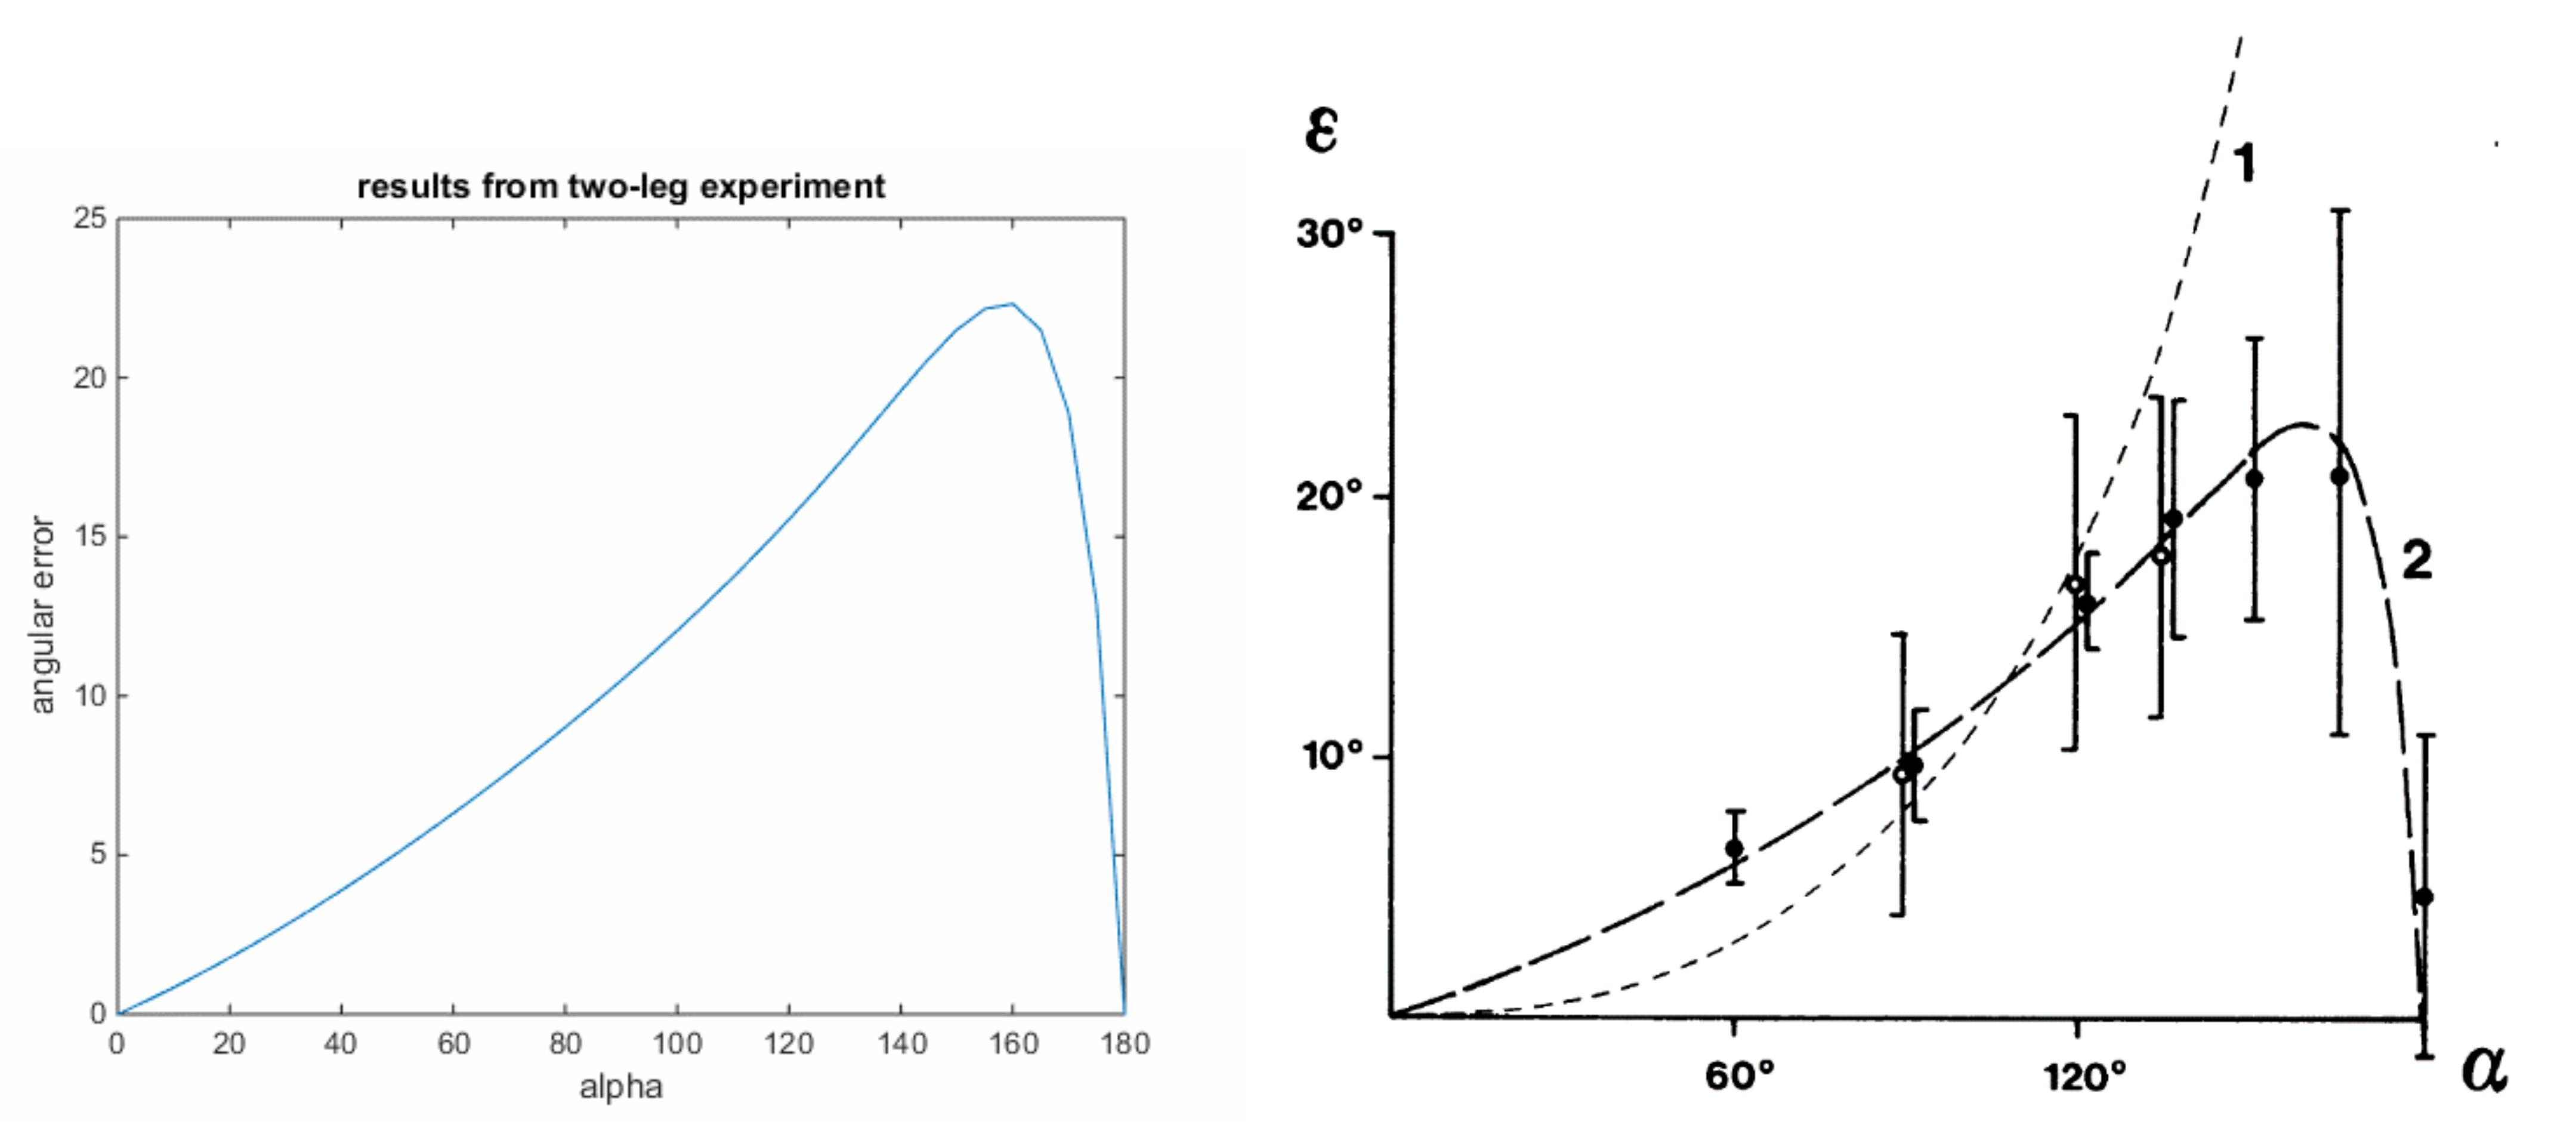
\includegraphics[scale=0.7]{./Pics/angularErrorCombined.png} 
\caption{Comparison }
\end{figure} 
}













\end{frame}










\end{frame}













\section{Local Orientation}
\begin{frame}
\frametitle{Local Orientation}
\begin{center}
Bla bla
\end{center}
\end{frame}

\section{Outlook}
\begin{frame}
\frametitle{Outlook and Conclusions}
\begin{center}
Bla bla
\end{center}
\end{frame}








\section{}
\begin{frame}
\frametitle{Thanks for your attention}
\begin{center}
Questions ?
\end{center}
\end{frame}


\end{document}